\subsubsection{Unstructured meshes}\label{unstructured-meshes}
% In the scientific and high performance communities concurrent operations on
% different meshes are commonly used; meshes can be used as discretisations to
% numerically solve partial differential equations (PDEs). Usually these
% simulations require millions of elements to get correct results. Structurally,
% we can differentiate between structured and unstructured meshes.\\
% Structured meshes have implicit connectivity between grid points: one can access neighbouring elements simply using indexing arithmetic without any further information.
% Structured applications consist of loops over blocks which access datasets
% defined on blocks and the access patterns required for an element is described
% by stencils. A part of a block and a stencil describing access shown in Figure
% \ref{fig:structured}. Most operations on structured grids can be easily
% parallelised even on GPUs since all nodes can be processed simultaneously.

% \begin{figure}
% \centering
% 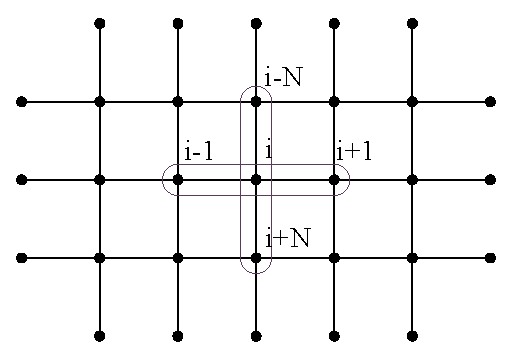
\includegraphics[width=4cm]{fig/svg/structured.eps}
% \caption{Structured mesh and stencil describing access pattern}
% \label{fig:structured}
% \end{figure}

In our work, we take a simple abstraction for describing unstructured meshes and computations on them. Unstructured meshes are defined by sets (e.g. nodes, edges, cells, etc.), data defined on the sets, and explicit connectivity information between sets (mapping tables). For determining the neighbours of a set element external information is needed - we need to access mapping tables. We represent sets as consecutive indexes from zero to the size of the set. The mapping between two sets is represented as a mapping table, an array which stores the index of set elements in the second set of the
mapping (referred as to-set) for every set element of the first set (from-set).
For the example in Figure \ref{fig:unstructured} a part of the mapping from
edges to cells is shown in Figure \ref{fig:mapping}. In this way we can access
the index of those elements which are connected to the current element of the
from-set from other sets (the to-sets of the mappings).

The computations on the mesh can commonly be given as a loop over the elements of a set, executing the same operations for every element, while accessing data directly on the iteration set or indirectly through a mapping. An example for a mesh and a mapping from
edges to cells are shown in Figure \ref{fig:unstructured}.


For our purposes, we classify computations into two categories. For kernels that
only access data directly or only read data indirectly but write the data on
the iteration set, the whole iteration space could run in parallel. However,
for kernels which indirectly increment data, we need to ensure that there are
no race conditions during the execution. The sole focus of our research is this second computational pattern. It is a pattern very common in finite volume and finite element applications: e.g. when updating state variables in cells using fluxes across faces, or when doing matrix assembly.

The parallelisation of such unstructured mesh operations is highly non-trivial: the exact race conditions cannot be determined from compile
time information, as they are driven by the mapping table.

\begin{figure}
\centering
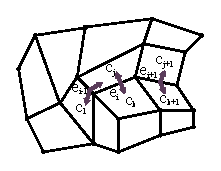
\includegraphics[width=4cm]{fig/svg/unstructured.eps}
\caption{Unstructured mesh, the arrow represents the mapping tells $e_i$ is
  connected to $c_j$ and $c_k$.}
\label{fig:unstructured}
\end{figure}



\begin{figure}
\centering
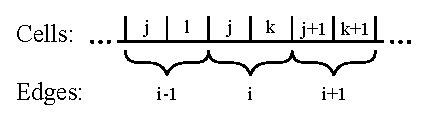
\includegraphics[width=6cm]{fig/svg/mapping.eps}
\caption{A part of the mapping from edges to cells.}
\label{fig:mapping}
\end{figure}

In our case we used some restrictions for the applications, but our work is
general enough that we are able to represent most applications in a way that
doesn't violate our restrictions. The first is that there is no data access
through multiple mappings. This means every piece of data that we access is either
defined directly on the iteration set, or it is accessed
through at most one level of indirection (a single mapping table entry). This restriction does not exclude applications
using nested indirections, since we can create a mapping that contains the
indexes that we access through multiple mapping. The second restriction is that
the result of the operations on the sets are independent from the order of
processing the elements of the sets. This restriction is necessary to ensure
that we can parallelise the operations, because there is no guarantee for
execution order in the parallelised versions. Finally, we only consider mappings with a fixed number of connections; such as edges to vertices (where the degree is always 2), unlike for a vertices to vertices mapping, where this will vary. The natural formalisation of most FEM and FV algorithm uses mappings with fixed number of connections.

